\begin{tcolorbox}[title=Problem 1, breakable]
    Graph each of the following partial sums of Fourier's expansion
    over the inverval $-1 \le x \le 3$.
    \begin{enumerate}
        \item $\frac{4}{\pi}\cos(\pi x/2)$
        \item $\frac{4}{\pi}(\cos(\pi x/2) - \frac{1}{3}\cos(3 \pi x/2))$
        \item $\frac{4}{\pi}(\cos(\pi x/2) - \frac{1}{3}\cos(3\pi x/2) + \frac{1}{5}\cos(5 \pi x/2))$
        \item $\frac{4}{\pi}(\cos(\pi x/2) - \frac{1}{3}\cos(3\pi x/2) + \frac{1}{5}\cos(5 \pi x/2)) - \frac{1}{7}\cos(7 \pi x/2))$
    \end{enumerate}
\end{tcolorbox}

\begin{figure}[h!]
    \centering
    \includegraphics[width=\textwidth]{images/chapter1/1.PNG}
\end{figure}

\newpage
\begin{tcolorbox}[title=Problem 2, breakable]
    Let $F_n(x)$ denote the sum of the first $n$ terms of the Fourier's series 
    evaluated at $x$:
    \[F_n(x) = \frac{4}{\pi}\left(\cos\frac{\pi x}{2} - \frac{1}{3}\cos\frac{3 \pi x}{2} + \cdots + \frac{(-1)^{n - 1}}{2n - 1}\cos\frac{(2n - 1)\pi x}{2}\right)\]
    \begin{enumerate}
        \item Evaluate $F_{100}(x)$ at $x = 0, 0.5, 0.9, 0.99, 1.1,$ and $2$. Is this close to the expected value?
        \item Evaluate $F_n(0.99)$ at $n = 100, 200, 300, \ldots, 2000$ and plot these successive approximations.
        \item Evaluate $F_n(0.999)$ at $n = 100, 200, 300, \ldots, 2000$ and plot these successive approximations.
        \item What is the value of this infinite series at $x = 1$?
    \end{enumerate}    
\end{tcolorbox}

\textbf{Solution (a):} I had no expectations.
\begin{enumerate}
    \item $F_{100}(0) = 0.9968169807056898$.
    \item $F_{100}(0.5) = 0.9954987558776579$.
    \item $F_{100}(0.9) = 0.9796927699334861$.
    \item $F_{100}(0.99) = 1.1789880778995547$
    \item $F_{100}(1.1) = -0.9796927699334861$.
    \item $F_{100}(2) = -0.9968169807056898$.
\end{enumerate}

\textbf{Solution (b):}
\begin{enumerate}
    \item $F_{100}(0.99) = 1.1789880778995547$
    \item $F_{200}(0.99) = 0.9028191668118976$
    \item $F_{300}(0.99) = 1.0661892530888835$
    \item $F_{400}(0.99) = 0.9499372563762823$
    \item $F_{500}(0.99) = 1.0402159950960959$
    \item $F_{600}(0.99) = 0.9664090460672992$
    \item $F_{700}(0.99) = 1.0288331847566468$
    \item $F_{800}(0.99) = 0.9747474084192721$
    \item $F_{900}(0.99) = 1.0224612312263757$
    \item $F_{1000}(0.99) = 0.9797755089505807$
    \item $F_{1100}(0.99) = 1.0183922416138902$
    \item $F_{1200}(0.99) = 0.9831360088728518$
    \item $F_{1300}(0.99) = 1.0155699566691612$
    \item $F_{1400}(0.99) = 0.9855398234944296$
    \item $F_{1500}(0.99) = 1.0134979445155288$
    \item $F_{1600}(0.99) = 0.9873443095081518$
    \item $F_{1700}(0.99) = 1.0119123060445154$
    \item $F_{1800}(0.99) = 0.9887486426910619$
    \item $F_{1900}(0.99) = 1.010659859489416$
    \item $F_{2000}(0.99) = 0.98987258246275$
\end{enumerate}

\begin{center}
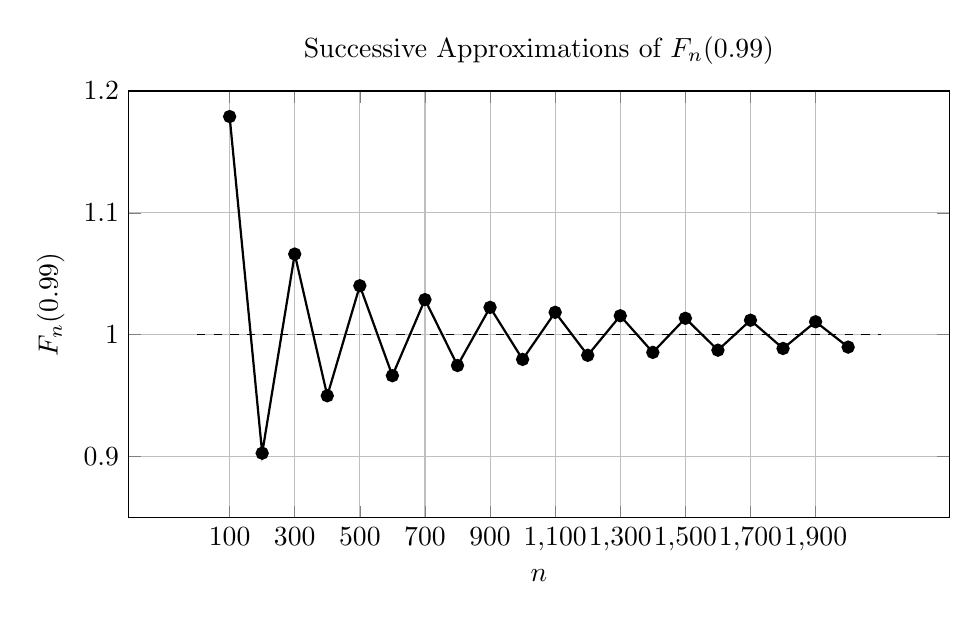
\begin{tikzpicture}
\begin{axis}[
    width=12cm,
    height=7cm,
    xlabel={$n$},
    ylabel={$F_n(0.99)$},
    title={Successive Approximations of $F_n(0.99)$},
    grid=both,
    ymin=0.85,
    ymax=1.2,
    xtick={100,300,500,700,900,1100,1300,1500,1700,1900}
]
\addplot[
    mark=*,
    thick
] coordinates {
    (100,1.1789880779)
    (200,0.9028191668)
    (300,1.0661892531)
    (400,0.9499372564)
    (500,1.0402159951)
    (600,0.9664090461)
    (700,1.0288331848)
    (800,0.9747474084)
    (900,1.0224612312)
    (1000,0.9797755090)
    (1100,1.0183922416)
    (1200,0.9831360089)
    (1300,1.0155699567)
    (1400,0.9855398235)
    (1500,1.0134979445)
    (1600,0.9873443095)
    (1700,1.0119123060)
    (1800,0.9887486427)
    (1900,1.0106598595)
    (2000,0.9898725825)
};
\addplot[dashed] coordinates {(0,1) (2100,1)};
\end{axis}
\end{tikzpicture}
\end{center}

\textbf{Solution (c):}
\begin{enumerate}
    \item $F_{100}(0.999) = 0.19890664596017577$
    \item $F_{200}(0.999) = 0.39133027939704734$
    \item $F_{300}(0.999) = 0.5711684699578463$
    \item $F_{400}(0.999) = 0.733053348578498$
    \item $F_{500}(0.999) = 0.8726544055639414$
    \item $F_{600}(0.999) = 0.9869094176114769$
    \item $F_{700}(0.999) = 1.074168253719476$
    \item $F_{800}(0.999) = 1.134240867961708$
    \item $F_{900}(0.999) = 1.1683479421219805$
    \item $F_{1000}(0.999) = 1.1789798278055126$
    \item $F_{1100}(0.999) = 1.1696760925989875$
    \item $F_{1200}(0.999) = 1.1447435828791337$
    \item $F_{1300}(0.999) = 1.10893505133833$
    \item $F_{1400}(0.999) = 1.0671127580619808$
    \item $F_{1500}(0.999) = 1.0239218847151361$
    \item $F_{1600}(0.999) = 0.9834971044374297$
    \item $F_{1700}(0.999) = 0.949222383157731$
    \item $F_{1800}(0.999) = 0.9235593491634196$
    \item $F_{1900}(0.999) = 0.9079537683550908$
    \item $F_{2000}(0.999) = 0.9028232919136085$
\end{enumerate}

\begin{center}
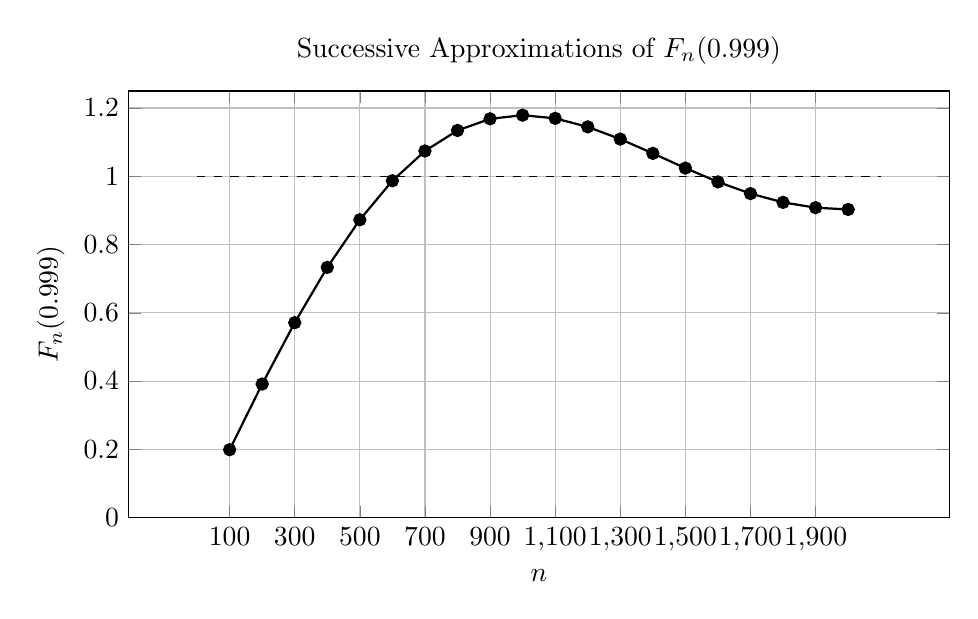
\begin{tikzpicture}
\begin{axis}[
    width=12cm,
    height=7cm,
    xlabel={$n$},
    ylabel={$F_n(0.999)$},
    title={Successive Approximations of $F_n(0.999)$},
    grid=both,
    ymin=0,
    ymax=1.25,
    xtick={100,300,500,700,900,1100,1300,1500,1700,1900}
]
\addplot[
    mark=*,
    thick
] coordinates {
    (100,0.1989066460)
    (200,0.3913302794)
    (300,0.5711684700)
    (400,0.7330533486)
    (500,0.8726544056)
    (600,0.9869094176)
    (700,1.0741682537)
    (800,1.1342408680)
    (900,1.1683479421)
    (1000,1.1789798278)
    (1100,1.1696760926)
    (1200,1.1447435829)
    (1300,1.1089350513)
    (1400,1.0671127581)
    (1500,1.0239218847)
    (1600,0.9834971044)
    (1700,0.9492223832)
    (1800,0.9235593492)
    (1900,0.9079537684)
    (2000,0.9028232919)
};
\addplot[dashed] coordinates {(0,1) (2100,1)};
\end{axis}
\end{tikzpicture}
\end{center}


\textbf{Solution (d):}
The value of the infinite series at $x = 1$ is $0$.

\begin{tcolorbox}[title=Problem 6, breakable]
    Fourier series illustrate the dangers of trying to find limits by simply substituting 
        the value that $x$ approaches. Consider the Fourier's series:
    \[f(x) = \frac{4}{\pi}\left(\cos\frac{\pi x}{2} - \frac{1}{3} \cos \frac{3 \pi x}{2} + \frac{1}{5} \cos \frac{5 \pi x}{2} - \frac{1}{7} \cos \frac{7 \pi x}{2} + \ldots\right)\]
    \begin{enumerate}
        \item What value does this approach as $x$ approaches $1$ from the left?
        \item What value does this approach as $x$ approaches $1$ from the right?
        \item What is the value at $f(1)$?
    \end{enumerate}
    These three answers are all different.
\end{tcolorbox}

\textbf{Solution (a):}
\[
\lim_{x \to 1^-} f(x) = 1.
\]
\textbf{Solution (b):}
\[
\lim_{x \to 1^+} f(x) = -1.
\]
\textbf{Solution (c):}
\[
f(1) = \frac{1 + (-1)}{2} = 0.
\]

\newpage
\begin{tcolorbox}[title=Problem 7, breakable]
    Consider the function that we get if we differentiate each summand of this function 
    $f(x)$ defined in equation $g(x) = -2\left(\sin \frac{\pi x}{2} - \sin \frac{2 \pi x}{2} + \sin \frac{5 \pi x}{2} - \sin \frac{7 \pi x}{2} + \cdots\right)$.
    \begin{enumerate}
        \item For $-1 < x < 3$, graph the partial sums of this series consisting of the first $10, 20, 30, 40,$ and $50$ terms.
              Does it appear that these graphs are approaching a constant function $0$.
        \item Evaluate the partical sums up to at least $20$ terms when $x = 0, 0.2, 0.3$, and $0.5$.
                 Does it appear that this series is approaching $0$ at each of these values of $x$/
        \item What \emph{is} happening at $x = 0, 0.2, 0.3, 0.5$? What can you prove?
    \end{enumerate}
\end{tcolorbox}

\textbf{Solution (a):}
\begin{enumerate}
\item $F_{10}(1.0) = -18.0$
\item $F_{20}(1.0) = -36.0$
\item $F_{30}(1.0) = -54.0$
\item $F_{40}(1.0) = -72.0$
\item $F_{50}(1.0) = -90.0$
\end{enumerate}
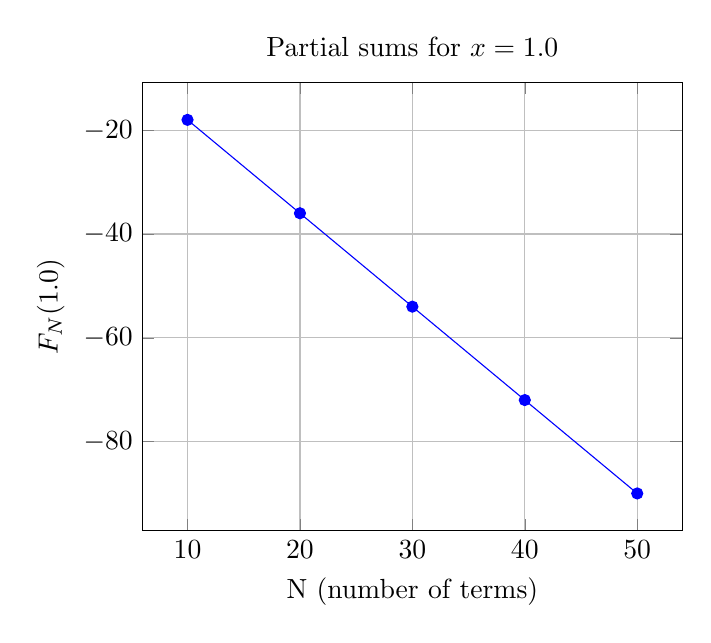
\begin{tikzpicture}
\begin{axis}[
    title={Partial sums for $x=1.0$},
    xlabel={N (number of terms)},
    ylabel={$F_N(1.0)$},
    xtick={10,20,30,40,50},
    ytick={-100,-80,-60,-40,-20,0},
    grid=major
]
\addplot[
    mark=*,
    color=blue
] coordinates {
    (10,-18.0)
    (20,-36.0)
    (30,-54.0)
    (40,-72.0)
    (50,-90.0)
};
\end{axis}
\end{tikzpicture}

\textbf{Solution (b):}

\begin{enumerate}
\item $F_{1}(0) = -0.0$
\item $F_{2}(0) = -0.0$
\item $F_{3}(0) = -0.0$
\item $F_{4}(0) = -0.0$
\item $F_{5}(0) = -0.0$
\item $F_{6}(0) = -0.0$
\item $F_{7}(0) = -0.0$
\item $F_{8}(0) = -0.0$
\item $F_{9}(0) = -0.0$
\item $F_{10}(0) = -0.0$
\item $F_{11}(0) = -0.0$
\item $F_{12}(0) = -0.0$
\item $F_{13}(0) = -0.0$
\item $F_{14}(0) = -0.0$
\item $F_{15}(0) = -0.0$
\item $F_{16}(0) = -0.0$
\item $F_{17}(0) = -0.0$
\item $F_{18}(0) = -0.0$
\item $F_{19}(0) = -0.0$
\item $F_{20}(0) = -0.0$
\end{enumerate}
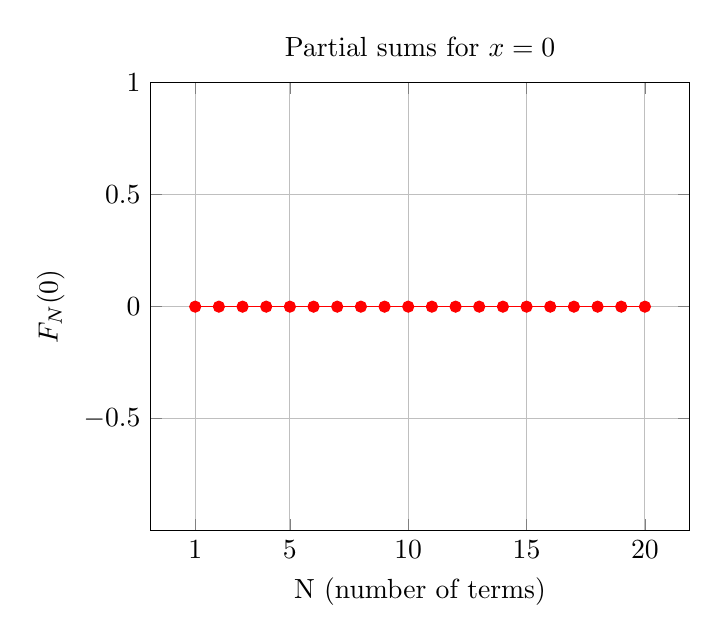
\begin{tikzpicture}
\begin{axis}[
    title={Partial sums for $x=0$},
    xlabel={N (number of terms)},
    ylabel={$F_N(0)$},
    xtick={1,5,10,15,20},
    grid=major
]
\addplot[
    mark=*,
    color=red
] coordinates {
    (1,-0.0) (2,-0.0) (3,-0.0) (4,-0.0) (5,-0.0)
    (6,-0.0) (7,-0.0) (8,-0.0) (9,-0.0) (10,-0.0)
    (11,-0.0) (12,-0.0) (13,-0.0) (14,-0.0) (15,-0.0)
    (16,-0.0) (17,-0.0) (18,-0.0) (19,-0.0) (20,-0.0)
};
\end{axis}
\end{tikzpicture}
\begin{enumerate}
\item $F_{1}(0.2) = -0.6180339887498948$
\item $F_{2}(0.2) = 0.5575365158350515$
\item $F_{3}(0.2) = -1.4424634841649486$
\item $F_{4}(0.2) = 0.17557050458494627$
\item $F_{5}(0.2) = -0.44246348416494874$
\item $F_{6}(0.2) = -1.0604974729148433$
\item $F_{7}(0.2) = 0.5575365158350525$
\item $F_{8}(0.2) = -1.4424634841649475$
\item $F_{9}(0.2) = 0.1755705045849465$
\item $F_{10}(0.2) = -0.44246348416494874$
\item $F_{11}(0.2) = -1.0604974729148435$
\item $F_{12}(0.2) = 0.11507303167010274$
\item $F_{13}(0.2) = -1.8849269683298973$
\item $F_{14}(0.2) = -0.26689297958000235$
\item $F_{15}(0.2) = -0.8849269683298974$
\item $F_{16}(0.2) = -1.502960957079792$
\item $F_{17}(0.2) = 0.11507303167010385$
\item $F_{18}(0.2) = -1.8849269683298961$
\item $F_{19}(0.2) = -0.26689297958000213$
\item $F_{20}(0.2) = -0.8849269683298974$
\end{enumerate}
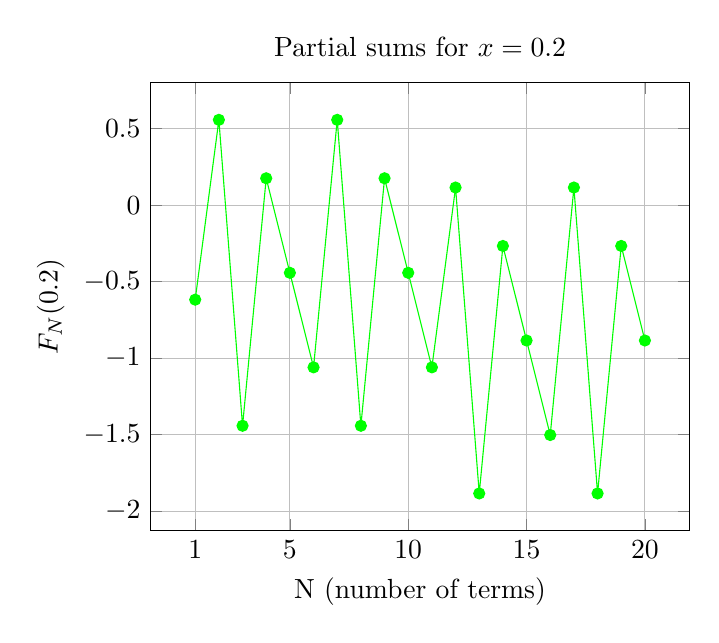
\begin{tikzpicture}
\begin{axis}[
    title={Partial sums for $x=0.2$},
    xlabel={N (number of terms)},
    ylabel={$F_N(0.2)$},
    xtick={1,5,10,15,20},
    grid=major
]
\addplot[
    mark=*,
    color=green
] coordinates {
    (1,-0.6180339887498948)
    (2,0.5575365158350515)
    (3,-1.4424634841649486)
    (4,0.17557050458494627)
    (5,-0.44246348416494874)
    (6,-1.0604974729148433)
    (7,0.5575365158350525)
    (8,-1.4424634841649475)
    (9,0.1755705045849465)
    (10,-0.44246348416494874)
    (11,-1.0604974729148435)
    (12,0.11507303167010274)
    (13,-1.8849269683298973)
    (14,-0.26689297958000235)
    (15,-0.8849269683298974)
    (16,-1.502960957079792)
    (17,0.11507303167010385)
    (18,-1.8849269683298961)
    (19,-0.26689297958000213)
    (20,-0.8849269683298974)
};
\end{axis}
\end{tikzpicture}
\begin{enumerate}
\item $F_{1}(0.3) = -0.9079809994790935$
\item $F_{2}(0.3) = 0.7100529892708014$
\item $F_{3}(0.3) = -0.7041605731022937$
\item $F_{4}(0.3) = -1.0170295031827552$
\item $F_{5}(0.3) = 0.7649835451939804$
\item $F_{6}(0.3) = -1.0170295031827563$
\item $F_{7}(0.3) = -0.7041605731022941$
\item $F_{8}(0.3) = 0.7100529892707993$
\item $F_{9}(0.3) = -1.265323691919476$
\item $F_{10}(0.3) = -0.3573426924403801$
\item $F_{11}(0.3) = -1.2653236919194737$
\item $F_{12}(0.3) = 0.3527102968304212$
\item $F_{13}(0.3) = -1.061503265542674$
\item $F_{14}(0.3) = -1.3743721956231354$
\item $F_{15}(0.3) = 0.4076408527536002$
\item $F_{16}(0.3) = -1.3743721956231365$
\item $F_{17}(0.3) = -1.0615032655426742$
\item $F_{18}(0.3) = 0.3527102968304192$
\item $F_{19}(0.3) = -1.622666384359856$
\item $F_{20}(0.3) = -0.7146853848807603$
\end{enumerate}
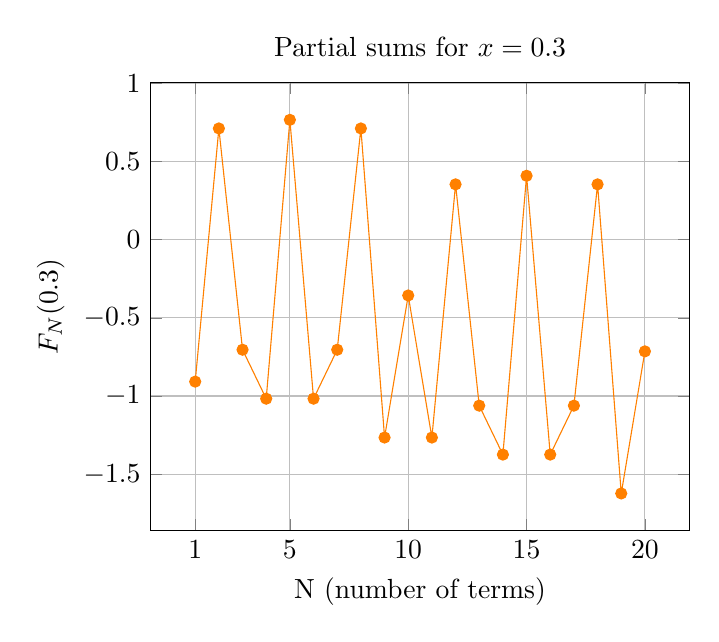
\begin{tikzpicture}
\begin{axis}[
    title={Partial sums for $x=0.3$},
    xlabel={N (number of terms)},
    ylabel={$F_N(0.3)$},
    xtick={1,5,10,15,20},
    grid=major
]
\addplot[
    mark=*,
    color=orange
] coordinates {
    (1,-0.9079809994790935)
    (2,0.7100529892708014)
    (3,-0.7041605731022937)
    (4,-1.0170295031827552)
    (5,0.7649835451939804)
    (6,-1.0170295031827563)
    (7,-0.7041605731022941)
    (8,0.7100529892707993)
    (9,-1.265323691919476)
    (10,-0.3573426924403801)
    (11,-1.2653236919194737)
    (12,0.3527102968304212)
    (13,-1.061503265542674)
    (14,-1.3743721956231354)
    (15,0.4076408527536002)
    (16,-1.3743721956231365)
    (17,-1.0615032655426742)
    (18,0.3527102968304192)
    (19,-1.622666384359856)
    (20,-0.7146853848807603)
};
\end{axis}
\end{tikzpicture}
\begin{enumerate}
\item $F_{1}(0.5) = -1.414213562373095$
\item $F_{2}(0.5) = 0.5857864376269051$
\item $F_{3}(0.5) = 2.0$
\item $F_{4}(0.5) = 0.5857864376269046$
\item $F_{5}(0.5) = -0.8284271247461901$
\item $F_{6}(0.5) = 0.5857864376269066$
\item $F_{7}(0.5) = 2.0000000000000027$
\item $F_{8}(0.5) = 0.5857864376269057$
\item $F_{9}(0.5) = -0.8284271247461898$
\item $F_{10}(0.5) = 0.5857864376269073$
\item $F_{11}(0.5) = -0.8284271247461876$
\item $F_{12}(0.5) = 1.1715728752538124$
\item $F_{13}(0.5) = 2.5857864376269073$
\item $F_{14}(0.5) = 1.171572875253812$
\item $F_{15}(0.5) = -0.24264068711928277$
\item $F_{16}(0.5) = 1.171572875253814$
\item $F_{17}(0.5) = 2.5857864376269095$
\item $F_{18}(0.5) = 1.1715728752538126$
\item $F_{19}(0.5) = -0.242640687119283$
\item $F_{20}(0.5) = 1.1715728752538141$
\end{enumerate}
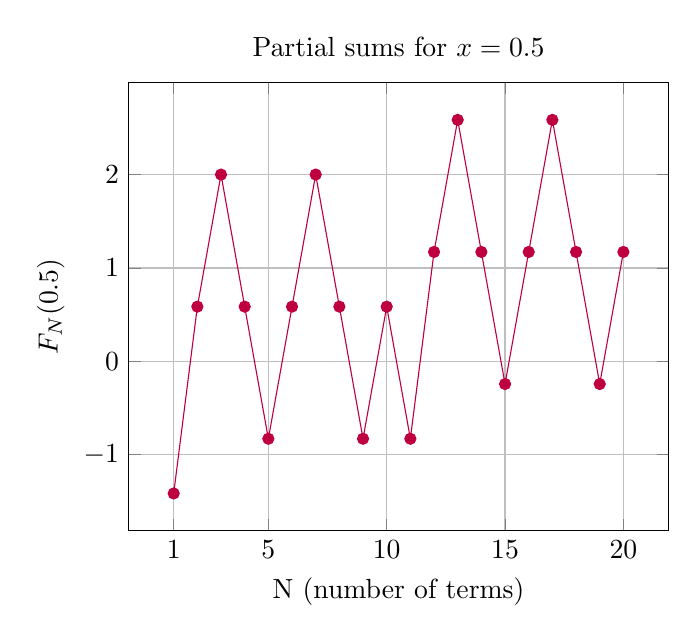
\begin{tikzpicture}
\begin{axis}[
    title={Partial sums for $x=0.5$},
    xlabel={N (number of terms)},
    ylabel={$F_N(0.5)$},
    xtick={1,5,10,15,20},
    grid=major
]
\addplot[
    mark=*,
    color=purple
] coordinates {
    (1,-1.414213562373095)
    (2,0.5857864376269051)
    (3,2.0)
    (4,0.5857864376269046)
    (5,-0.8284271247461901)
    (6,0.5857864376269066)
    (7,2.0000000000000027)
    (8,0.5857864376269057)
    (9,-0.8284271247461898)
    (10,0.5857864376269073)
    (11,-0.8284271247461876)
    (12,1.1715728752538124)
    (13,2.5857864376269073)
    (14,1.171572875253812)
    (15,-0.24264068711928277)
    (16,1.171572875253814)
    (17,2.5857864376269095)
    (18,1.1715728752538126)
    (19,-0.242640687119283)
    (20,1.1715728752538141)
};
\end{axis}
\end{tikzpicture}

\textbf{Solution (c):}
At $x=0$, the series converges to $0$. 
At $x=0.2,0.3,0.5$, the partial sums oscillate and do not settle to $0$ quickly.